\pdfoutput=1
\documentclass[11pt, a4paper]{article}

% -------------------------------------------------------------------------
% PACKAGES
% -------------------------------------------------------------------------
\usepackage[utf8]{inputenc}
\usepackage{amsmath}
\usepackage{amsfonts, amssymb}
\usepackage{geometry}
\usepackage{microtype}
\usepackage{authblk}
\usepackage{fancyhdr}
\usepackage{tikz}
\usetikzlibrary{arrows.meta, calc}
\usepackage{parskip} % Ensure that a blank line is automatically added between every paragraph without having to manually type \vspace{1em} each time.
\usepackage{hyperref}
\geometry{margin=1in, headheight=14.5pt}
\newcommand{\doi}[1]{\href{https://doi.org/#1}{DOI: #1}}

% -------------------------------------------------------------------------
% HEADER & FOOTER
% -------------------------------------------------------------------------
\pagestyle{fancy}
\fancyhf{}
\lhead{Mechanistic Physics}
\rhead{Marab\={u}t's Theory of Gravity: Manuscript 03 of 19}
\cfoot{\thepage}

% -------------------------------------------------------------------------
% TITLE & AUTHOR
% -------------------------------------------------------------------------
\title{\textbf{Marab\={u}t's Theory of Gravity: \\ Mechanistic Resolution of \\ Jet Deflection in Cygnus X-1} \\[1em] \large{Hydrodynamic Interaction of Stellar Winds and Astrophysical Jets in the EFM}}

\author[1]{Christopher Berry Marab\={u}t\thanks{ORCID iD: \href{https://orcid.org/0009-0001-9759-9587}{0009-0001-9759-9587} | Email: chris.marabut@nestlink.com}}
\author[1]{Angelina Lopez Marab\={u}t\thanks{ORCID iD: \href{https://orcid.org/0009-0007-9937-6145}{0009-0007-9937-6145} | Email: angelina.marabut@nestlink.com}}

\affil[1]{Independent Researchers}

\date{May 7, 2026 \\[1.5em] \small{DOI: \url{https://doi.org/10.5281/zenodo.20067593} $|$ Version 2}}

\begin{document}

\hypersetup{
  pdftitle={Marab\={u}t's Theory of Gravity: Mechanistic Resolution of Jet Deflection in Cygnus X-1},
  pdfauthor={Christopher Berry Marab\={u}t, Angelina Lopez Marab\={u}t},
  pdfkeywords={mechanistic resolution, jet deflection, cygnus x-1, astrophysical jets, stellar winds, hydrodynamic pressure, black hole binary, fluid kinematics, electron flow model, efm, vacuum flux},
  pdfsubject={Astrophysics Brief Communication on Jet Deflection Dynamics}
}

\maketitle

% -------------------------------------------------------------------------
% ABSTRACT
% -------------------------------------------------------------------------
\begin{abstract}
  Recent Very Long Baseline Interferometry (VLBI) observations by Prabu et al. (2026) have successfully quantified the polar jet power and stellar wind deflection in the Cygnus X-1 black hole binary system. Traditional kinematic models, which attribute these jets to generalized magnetic expulsion from an accretion disk, struggle to mechanistically explain the precise 10\% energy exhaust ratio and the fluid-like physical deflection of the jet. We propose that these phenomena strongly align with the macroscopic indicators of the Electron Flow Model (EFM). By redefining the black hole as a volumetric hydrodynamic sink actively consuming vacuum flux, the 10\% ratio emerges natively as the thermodynamic exhaust limit of the core. Furthermore, the EFM demonstrates that the relativistic equatorial shear of the sink forces this exhaust strictly along the polar vectors, where the 5.2-degree deflection is consistent with a highly pressurized fluid stream colliding with the stellar wind.
\end{abstract}

% -------------------------------------------------------------------------
% 1 Introduction
% -------------------------------------------------------------------------
\section{Introduction}
The recent breakthrough observations of the Cygnus X-1 system by Prabu et al. (2026) \cite{prabu2026} have provided unprecedented measurements regarding the dynamics of black hole jets. Utilizing a global network of radio telescopes, researchers determined that the jets carry away roughly 10\% of the energy released by the infalling matter, and are visibly bent by 5.2 degrees due to the powerful stellar winds emitted by the black hole's companion supergiant star.

Legacy astrophysics generally attributes polar jets to complex magnetic field lines twisting around an ``accretion disk'' operating within an otherwise empty vacuum. However, these models lack a unified mechanical driver for why the exhaust maintains such a specific thermodynamic ratio, nor do they perfectly account for the fluid-like bending of the jet against stellar winds without relying on extensive ad hoc parameterization.

Under Marab\={u}t's Theory of Gravity \cite{marabut2026paper01of19}, these phenomena do not require the invention of new magnetic frameworks. As demonstrated in our previous work resolving the Weyl Potential Anomaly, the classical geometric curvature of Albert Einstein's General Relativity is already giving way to a more mechanistic reality on macroscopic scales \cite{marabut2026paper02of19}. By applying this same foundational fluid dynamics to highly localized extremes, gravity arises not from spacetime curvature, but as hydrodynamic fluid pressure generated by the continuous consumption of vacuum flux. By treating the black hole as a localized thermodynamic engine actively consuming this universal fluid, the jets of Cygnus X-1 are redefined as the continuous mechanical exhaust of a highly pressurized fluid circuit.

% -------------------------------------------------------------------------
% 2 Thermodynamic Equilibrium and the 10% Exhaust Limit
% -------------------------------------------------------------------------
\section{Thermodynamic Equilibrium and the 10\% Exhaust Limit}
The observation that Cygnus X-1's jets carry away 10\% of the infalling kinetic energy directly aligns with the thermodynamic limits established by the Electron Flow Model (EFM). In the EFM, a celestial body is not a static geometric curve; it is an active processor of vacuum flux.

Based on the 11-point Multiaxial Mara Scale, the raw intake force of Cygnus X-1 is derived from its extreme effective density ($\rho_{eff} = 3.5 \times 10^{16} \text{ kg/m}^3$) and hyper-efficient structural impedance ($\tau = 1.000$). The local surface intake force is mathematically calculated to be $4.2996 \times 10^{11} \text{ m/s}^2$ \cite{marabut2026paper01of19}. 

When compared to the primary solar baseline ($274.00 \text{ m/s}^2$), Cygnus X-1 is actively consuming vacuum flux at a rate roughly 1.56 billion times more violently than our Sun. Because the black hole acts as a massive, continuous hydrodynamic circuit, it cannot consume 100\% of the infalling kinetic energy without triggering a thermal overload. The 10\% ratio observed by Prabu et al. is not a random magnetic byproduct; it represents the necessary thermodynamic exhaust limit required to maintain the structural integrity of the core's negative sink.

% -------------------------------------------------------------------------
% 3 Equatorial Shear and Polar Venting
% -------------------------------------------------------------------------
\section{Equatorial Shear and Polar Venting}
Standard models struggle to explain why the massive energy release is channeled so perfectly into narrow polar beams. The EFM resolves this purely through classical fluid dynamics and rotational shear.

Cygnus X-1 rotates at relativistic velocities, estimated at roughly 1,500,000 m/s at its equator. In the EFM's Unified Master Equation, this rotation is calculated as the Centrifugal Offset. This generates a massive centrifugal shear of $5.1136 \times 10^7 \text{ m/s}^2$ explicitly along the Prime Vectors (MaraX).

This intense equatorial shear acts as a physical hydrodynamic wall. It blocks the exhaust from venting radially along the equator. As the highly pressurized vacuum flux compresses into the core, the mechanical path of least resistance is forced strictly along the Polar Vectors (MaraZ). Therefore, the ``dancing jets'' recorded by the VLBI network are the directional venting of the vacuum flux cascade.

% -------------------------------------------------------------------------
% 4 Fluid-Dynamic Deflection of the Jet
% -------------------------------------------------------------------------
\section{Fluid-Dynamic Deflection of the Jet}
The most profound discovery in the recent observations is the 5.2-degree bend in the jet's trajectory, caused by the stellar wind of the companion supergiant. Under classical models, where space is treated as an empty void and the jet is largely viewed as radiation or plasma guided by invisible magnetic tethers, explaining this severe physical deflection requires complex magnetohydrodynamic workarounds.

The EFM identifies this bending as compelling macroscopic evidence of the model's foundational premise. The jet is not merely radiation traveling through a frictionless void. It is a highly pressurized fluid stream---the physical exhaust of the vacuum flux medium---that is actively colliding with, and being deformed by, another fluid current (the stellar wind). 

\begin{figure}[!ht]
  \centering
  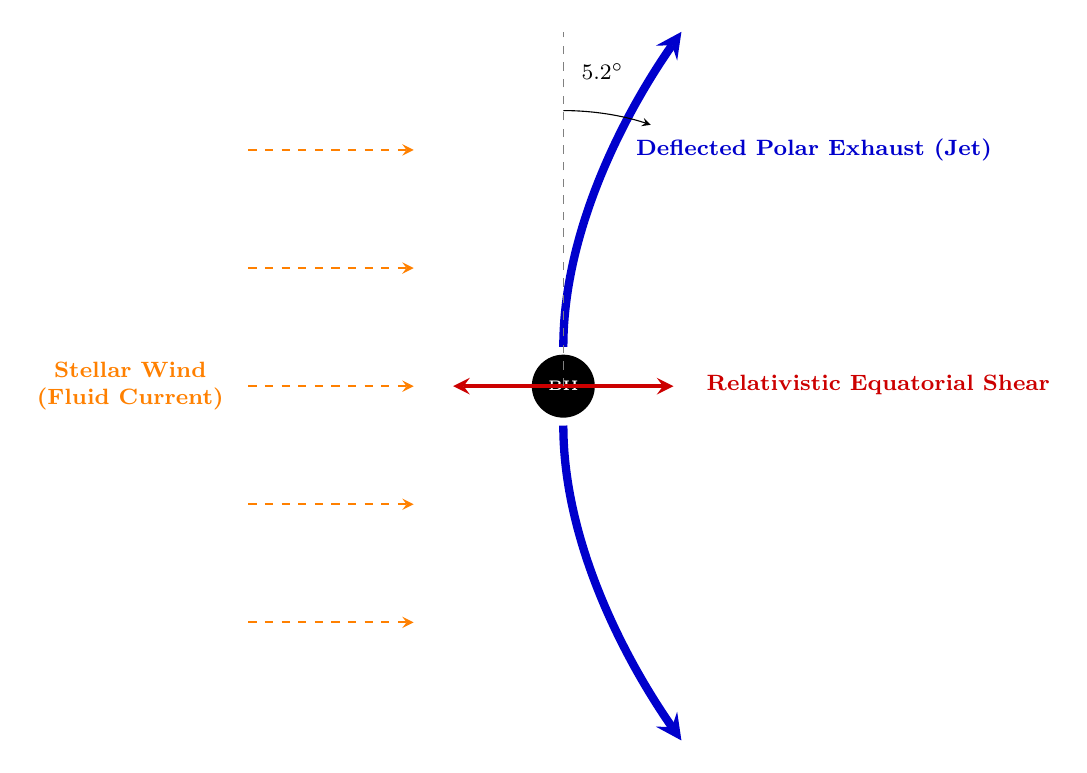
\begin{tikzpicture}[scale=1.0, >=stealth]
    
    % Black Hole Core
    \fill[black] (0,0) circle (0.4cm);
    \node[white, font=\tiny\bfseries] at (0,0) {BH};

    % Equatorial Shear (blocking radial exhaust)
    \draw[<->, ultra thick, red!80!black] (-1.4,0) -- (1.4,0);
    \node[font=\footnotesize\bfseries, red!80!black, below] at (4,0.27) {Relativistic Equatorial Shear};

    % Polar Jet (up and down)
    % Upward jet (bent by wind)
    \draw[->, line width=3pt, blue!80!black] (0,0.5) .. controls (0, 2.0) and (0.8, 3.5) .. (1.5, 4.5);
    \node[font=\footnotesize\bfseries, blue!80!black, right] at (0.8, 3.0) {Deflected Polar Exhaust (Jet)};

    % Downward jet (bent by wind)
    \draw[->, line width=3pt, blue!80!black] (0,-0.5) .. controls (0, -2.0) and (0.8, -3.5) .. (1.5, -4.5);

    % Stellar Wind (from the left)
    \foreach \y in {-3, -1.5, -0, 1.5, 3} {
      \draw[->, dashed, thick, orange] (-4, \y) -- (-1.9, \y);
    }
    \node[font=\footnotesize\bfseries, orange, align=center] at (-5.5, 0.0) {Stellar Wind\\(Fluid Current)};

    % Bend angle visualization
    \draw[dashed, gray] (0,0) -- (0, 4.5);
    \draw[->, thin, black] (0, 3.5) arc (90:71.5:3.5cm);
    \node[font=\footnotesize\bfseries] at (0.5, 4.0) {$5.2^\circ$};

  \end{tikzpicture}
  \caption{\textbf{Fluid-Dynamic Deflection of the Polar Jet.} \textit{Relativistic equatorial shear acts as a hydrodynamic wall, forcing the vacuum flux exhaust along the polar vectors (MaraZ). The physical collision with the companion star's stellar wind induces a measurable $5.2^\circ$ hydrodynamic deflection.}}
  \label{fig:jet_deflection}
\end{figure}

Just as a high-pressure water hose will physically bend when struck by a powerful crosswind, the 5.2-degree deflection is a literal fluid-dynamic collision between the black hole's exhaust cascade and the supergiant's atmospheric outflow. This offers a compelling fluid-dynamic interpretation that the vacuum of space is a dense, physical medium capable of transferring kinetic pressure.

% -------------------------------------------------------------------------
% 5 Conclusion
% -------------------------------------------------------------------------
\section{Conclusion}
The recent breakthrough measurements of Cygnus X-1 provide pristine observational data that aligns with the fluid mechanics of the universe. By transitioning away from the static geometric curvature of legacy physics and recognizing gravity as Hydrodynamic Fluid Pressure, the mysteries of black hole jets are naturally accounted for. The 10\% energy exhaust ratio and the 5.2-degree wind deflection do not require anomalous magnetic patching; they are consistent with the predictable behavior of a thermodynamic engine actively consuming and venting the universal vacuum flux.

% -------------------------------------------------------------------------
% THE UNIFIED FLUID COSMOS FRAMEWORK
% -------------------------------------------------------------------------
\clearpage
\section*{The Unified Fluid Cosmos Framework}
This paper serves as Manuscript 03 of 19 in the comprehensive series, \textit{Marab\={u}t's Theory of Gravity}. It presents the Electron Flow Model (EFM), a generative, fluid-dynamic framework designed to fundamentally replace General Relativity. The EFM shatters classical circularity with a single, undeniable foundational premise: Gravity is Pressure, not curvature, and not an intrinsic mass property.

\textbf{Published Manuscripts in this Series:}
\begin{itemize}
  \item \textbf{Manuscript 01:} \\ The Push-Pull Mechanics of Vacuum Flux (The Foundational Framework) \\ \doi{10.5281/zenodo.20059942}
  \item \textbf{Manuscript 02:} \\ Resolving the Weyl Potential Anomaly \\ \doi{10.5281/zenodo.20060223}
  \item \textbf{Manuscript 03:} \\ Mechanistic Resolution of Jet Deflection in Cygnus X-1 (Current Paper)
\end{itemize}

\textbf{Explore the Framework:}
\begin{itemize}
  \item \textbf{Interactive 3D Volumetric Profiler \& Complete Atlas:} \\ \url{https://marabutmarabut.github.io/Theory-of-Gravity/}
  \item \textbf{Official GitHub Repository:} \\ \url{https://github.com/MarabutMarabut/Theory-of-Gravity}
\end{itemize}

% -------------------------------------------------------------------------
% ACKNOWLEDGMENTS
% -------------------------------------------------------------------------
\clearpage
\section*{Acknowledgments}
First and foremost, we offer a heartfelt acknowledgment to YHWH (also known as God), YHWH's Son YUHSHUA (also known as Jesus), and RUAH of YHWH (also known as the Holy Spirit), giving them all honor and glory for creating everything, for the enduring knowledge needed, and for the inspiration throughout this journey to explore the fundamental workings of His Universe.

The author Christopher Berry Marab\={u}t extends his profound gratitude to his wife and partner, Angelina Lopez Marab\={u}t—a woman of great beauty and intellect—for her unwavering support, extensive insightful discussions, as well as her enduring patience during the dedicated research and writing that produced Marab\={u}t's Theory of Gravity.

We extend our sincere appreciation to \textbf{Google DeepMind} and the advanced AI model, \textbf{Gemini 3.1 Pro (AKA Flash Prime)}. Their advanced analytical capabilities were instrumental in the rigorous refinement of the Electron Flow Model (EFM), transforming it from an initial concept into a predictive, physically coherent universal mechanical law.

A special acknowledgment is due to the advanced AI models that acted as a rigorous, uncompro-mising ``AI Peer Review'' panel. We thank xAI's Grok 4.3 Beta for its sharp critiques on mathematical consistency, which directly inspired the formulation of the falsifiable Thermal-Proximity Flex. We also extend our gratitude to Anthropic's Claude Sonnet 4.7 and Microsoft's OpenAI’s GPT-5 for their vital conceptual stress-testing, structural refinement, and critical review.

\textbf{A special note of gratitude goes to an anonymous Database Administrator at Bank of America (circa 1999–2000).} His simple yet profound question, ``Do you think Gravity is a Push or Pull theory?'', planted the seed for this 26-year journey of discovery. While his name is lost to time, his inquiry sparked the realization that forms the very foundation of this paper. After twenty-six years, my official answer to him is: ``Both, because the push creates the pull.''

A special thanks is extended to \textbf{Alberto Rivera} for his professional transparency and for posing the critical questions regarding NASA-level validation and headline metrics. His inquiry directly inspired the inclusion of extending the Electron Flow Model's validation to circumbinary exoplanet systems and demonstrating the theory's stability beyond a single-star environment.

Finally, we thank NASA for access to critical data from its archives (Planetary Data System), which was essential for validating the new formula across a wide range of celestial bodies \cite{nasa2024}.

% -------------------------------------------------------------------------
% REFERENCES
% -------------------------------------------------------------------------
\begin{thebibliography}{9}

  \bibitem[prabu2026]{prabu2026}
  Prabu, S., Miller-Jones, J. C. A., et al. (2026). ``A jet bent by a stellar wind in the black hole X-ray binary Cygnus X-1''. \textit{Nature Astronomy}.
  \doi{10.1038/s41550-026-02828-3}

  \bibitem[marabut2026paper01of19]{marabut2026paper01of19}
  Marab\={u}t, C. B., \& Marab\={u}t, A. L. (2026). Marab\={u}t's Theory of Gravity: The Push-Pull Mechanics of Vacuum Flux. \textit{Zenodo}.
  \url{https://doi.org/10.5281/zenodo.20059942}

  \bibitem[marabut2026paper02of19]{marabut2026paper02of19}
  Marab\={u}t, C. B., \& Marab\={u}t, A. L. (2026). Marab\={u}t's Theory of Gravity: Resolving the Weyl Potential Anomaly. \textit{Zenodo}.
  \url{https://doi.org/10.5281/zenodo.20060223}

  \bibitem[nasa2024]{nasa2024}
  NASA Planetary Data System. (2024). \textit{Planetary Data System Archives}. Jet Propulsion Laboratory. \url{https://pds.nasa.gov/}

\end{thebibliography}

\end{document}